%!TeX root=../main.tex
\فصل{طراحی بردمدارچاپی}
\قسمت{مقدمه}
بردمدارچاپی\پانویس{Printed Circuit Board (PCB)} بردی است که با کانکتور و ترک‌هایی که روی آن قرار دارد قطعات را به‌طور الکتریکی به یکدیگر متصل می‌کند. بردمدارچاپی به‌طورکلی متشکل از هسته‌ای محکم معمولاً از جنس فیبرشیشه \متن‌لاتین{FR4} و لایه‌های مسی نازک که در یک یا دو طرف آن قرار دارند می‌شود. ترک‌ها و پدها روی لایه‌های مسی و پس از حل کردن مس سایر بخش‌ها در اسید به وجود می‌آیند. برای محافظت از تماس ناخواسته ترک‌های مسی با قطعات و ذرات رسانا و همچنین جدا نمودن محل‌های لحیم‌کاری از سایر بخش‌ها، بر روی لایه مسی لایه‌ی \متن‌لاتین{Solder mask} قرار می‌گیرد که معمولاً به رنگ سبز است.

یکی از موارد مهم در مرحله طراحی‌بردمدارچاپی توجه به تأثیرات نویز در مدار و تلاش به کاهش اثرات آن است. نویزها می‌تواند به دو صورت الکتریکی (در اثر خاصیت خازنی بین دو هادی) و مغناطیسی (در اثر خاصیت سلفی هادی) به وجود بیایند. منابع اصلی نویز سیگنال‌های پرودیک با فرکانس بالا نظیر زوج سیم‌های تفاضلی (\متن‌لاتین{D+} و \متن‌لاتین{D-} موجود در \متن‌لاتین{USB}) یا سیگنال‌های ساعت\پانویس{Clock} هستند. 

با عبور جریان از یک هادی میدان مغناطیسی در اطراف آن به وجود می‌آید و در صورت وجود هادی‌ای دیگر در نزدیکی آن میدان تولیدشده روی آن تأثیر گذاشته و باعث ایجاد جریان در هادی دوم می‌شود. همچنین وجود اختلاف‌پتانسیل بین دو هادی مجاور سبب ایجاد میدان الکتریکی شده و تغییرات پتانسیل یک هادی روی دیگری همانند صفحات یک خازن اثر می‌گذارد. کاهش طول هادی‌ها یکی از عوامل مؤثر در کاهش این نوع نویزها است. استفاده از خازن‌های کوپلاژ برای میکروکنترلر \مرجع{AN2586}، استفاده از فیلترهای \متن‌لاتین{RC} و \متن‌لاتین{LC}، استفاده از \متن‌لاتین{Polygon} (یا \متن‌لاتین{Pour}) و استفاده از انواع شیلد و محافظ‌های زمین شده، از روش‌ها کاهش انواع نویز هستند که در طراحی بردمدار چاپی باید به آن‌ها توجه کرد. بردهای این پروژه نیز مطابق با این نکات طراحی‌شده‌اند.



\قسمت{ملاحظات طراحی \متن‌لاتین{PCB}}
در گذشته فرکانس سیستمها از حد چند مگاهرتز تجاوز نمیکرد و برد های مدار چاپی یک یا دو لایه تنها به عنوان بستری جهت قرار دادن المانها و برقراری ارتباط بین آنها مورد استفاده قرار می گرفت. همچنین نحوه اتصال و قرار گیری المانها و مسیر ها تاثیری در کارایی سیستم نداشت.

عوامل تاثیر گذار در بازنگری نحوه طراحی سیستم های جدید\\ 
1- کاهش ابعاد المانهای مدار و فاصله ی بین آنها \\
2- کاهش عرض مسیر سیگنالها و فاصله بین آنها \\
3- کاهش ولتاژ تغذیه سیستم و افزایش جریان آن\\
4- کاهش حاشیه نویز\\
5- افزایش فرکانس و نرخ انتقال اصلاعات در سیستم های دیجیتال\\
6- المان های سوئیچینگ با جریان بالا\\
7- تراشته هایی با تعداد پایه های وروی – خروجی زیاد

اغلب طراحان دیجیتال، سیستم را در حوزه و زمان و با توجه به پارامتر هایی از قبیل زمان صعود سیگنال یا تاخیر انتشار توصیف میکند در حالیکه جهت تحلیل و بررسی بسیاری از پدیده ها در سیستم های آنالوگ از حوزه فرکانس استفاده می شود.

کاهش ابعاد سیستم های طراحان برد های الکترونیکی را بر آن واداشته است که المانها و مسیر سیگنالها را در کمترین فاصله ممکن از یکدیگر قرار دهند که همین امر موجب شده است اثر متقابل میدان های الکتریکی و مغناطیسی تولید شده توسط اجزای مختلف مدار بیش از قبل مورد توجه قرار گیرد. اتصال بین المانهای مختلف سیستم از مبدا تا مقصد توسط سیم، کابل یا مسیرهای موجود به روی برد برقرار میشود. در فرکانس های پایین می توان این مسیرها رو به صورت ایده آل در نظر گرفت.

اما همانگونه که در شکل مشاهده میشود با افزایش فرکانس، هاصیت سلفی و خازنی و مقاومتی مسیر اثر خود را نشان می دهد. لازم است طراحی سیستم مورد توجه قرار گیرد زیرا امپدانس ایجاد شده توسط این المانها به تضعیف سیگنال در فرکانس های بالا منتهی می شود.
به این ترتیب با افزایش فرکانس، اثرات سلفی و خازنی المانهای مدار که در فرکانسهای پایین از آنها صرفنظر میشود، قابل چشم پوشی نمی باشد و مسیر های اتصال دهنده المانها به روی برد سیستم، به صورت مجموعه ای از سلفها و خازنها مدلسازی میشود که این مدل، خط انتقال نامیده میشود.\\
نکته: باید توجه داشت که بر خلاف تصور رایج تنها فرکانس سیگنالها عامل تعیین کننده نمی باشد بلکه زمان نزول و صعود سیگنال نیز معیار تصمیم گیری است. به عنوان مثال طراحی سیستمی با فرکانس کاری 100MHZ و زمان صعود و نزول 2ns ساده تر از طراحی و نزول 1ns می باشد.

در سیستمهای مرکب که از دو بخش دیجیتال و آنالوگ تشکیل شده اند مشکلات دیگری نیز وجود دارد. به عنوان مثال در مورد مبدل های آنالوگ به دیجیتال پیشرفته، انرژی سیگنال در سمت دیجیتال ممکن است 130 db بیشتر از انرژی سیگنال در سمت آنالوگ باشد، به این ترتیب نویز موجود در قسمت دیجیتال، ورودی آنالوگ را به شدت تحت تاثیر قرار می دهد و باید از روش های مناسب به منظور کاهش این اثرات استفاده نمود.\\
از سوی دیگر با پیشرفت تکنولوژی ساخت ادوات نیمه هادی، تعداد پایه های خارجی تراشه ها و حجم گیت های داخلی آنها ، اقزایش چشم گیری داشته است.\\
همچنین با اقزایش سرعت پردازش سیستم از چند مگاهرتز به چند گیگاهرتز، مصرف جریان دینامیک تراشه ها چندین برابر شده است. با توجه به آنکه نویز ایجاد شده در سیستم مطابق با رابطه L*di/dt، با سرعت و مقدار تغییرات جریان متناسب است عوامل فوق به افزایش نویز تولید شده منتهی میشود.\\
با کاهش ولتاژ تغذیه سیتم از 5v به مقادیر 1.2v، 1.8v، 2.5v، حساسیت تراشه ها به نویز سیستم نیز بیش از پیش افزایش یافته است که عدم توجه به موارد فوق در هنگام طراحی، به عملکرد نامطلوب سیستم منتهی خواهد شد.

با توجه به مطالب عنوان شده شناخت پدیده های ایجاد شده در فرکانس های بالا از قبیل اثر سیکنال ها به روی یکدیگر تغییر ولتاژ سیگنال مرجع و بررسی راه حل های از قبیل کنترل امپدانس، مسیرکشی صحیح سیگنالهای آرایش صحیح لایه ها در برد های مدار چاپی و طراحی صحیح سیتم تغذیه از جمله مواردی هستند که به منظور حذف یا کاهش اثر پدیده های فوق در فرکانس های بالا مورد توجه می باشد.

\زیرقسمت{خطوط انتقال}

با افزایش فرکانس لازم است اثرات خطوط انتقال سیگنال در طراحی سیستم مورد توجه قرار گیرد به این ترتیب در صورتی که طول مسیر سیگنال به روی برد مدار چاپی تا حدی افزایش یابد تا زمان لازم جهت رفت و برگشت سیگنال در طول مسیر قابل مقایسه با زمان صعود یا نزول آن باشد، لازم است محاسبات خطوط انتقال در طراحی مورد توجه قرار گیرد.

عدم تطابق بین انپدانس نشخصه خط انتقال با امپدانس خروجی در درایور یا امپدانس ورودی بار به بازتابش سیگنال منتهی می شود. این باز تابش ها به اعوجاج سیگنال و بروز فرا جهش یا فرو جهش در شکل موج آنها می انجامد که در سیستم های آسنکرون ممکن است تغییرات ناخواسته سیگنال و عملکرد ناصحیح سیستم را در پی داشته باشد.

 \زیرزیرقسمت{نتیجه‌گیری}
 
کلیه مسیرها توسط باری برابر با امپدانس مشخصه خط پایان دهی شوند.\\
مسیر سیگنالهای فرکانس بالا با توجه به اصول خط انتقال طراحی شود.\\
تغییر امپدانس مسیر می تواند بر اثر هر یک از عوامل زیر رخ دهد:\\
1- تغییر عرض مسیر سیگنال\\
2- قرار ادن via در میسیر سیگنال و تغییر لایه آن \\
3- عبور از کانکتور \\
4- انشعابات ایجاد شده در مسیر سیگنال\\

\زیرقسمت{اندازه گیری بازتابش سیگنالها }

به منظور اندازه گیری باز تابش سیگنالها نرم افزارهای متعددی ارئه شده است که میتوان با شبیه سازی خط انتقال و مدلسازی آن، سیگنال مناسب را به خط انتقال اعمال کرد و نحوه بازتابش سیگنال در نقاط مختلف را بررسی نمود. علاوه بر نرم افزارهای موجود از وسیله ای به نام TDR استفاده می شود.

بر اسای مطالب گفته شده علت اصلی بازتابش سیگنالها عدم تطبیق امپدانس مشخصه خط انتقال با امپدانس فرستنده و گیرنده می باشد به این ترتیب با رفع این مشکل میتوان اثر پدیده های ناشی از بازتابش سیگنالها را تا حد زیادی کاهش داد. در ادامه روشهای موجود جهت تطبیق امپدانس خط انتقال با مشخصات فرستنده و گیرنده را مورد بررسی قرار میدهیم.

\زیرزیرقسمت{پایان دهی موازی}
در این روش مقاومتی برابر با امپدانس مشخصه خط به انتهای مسیر متصل می شود. به این ترتیب کلیه انرژی سیگنال توسط مقاومت جذب می شود و هیچگونه بازتابش سیگنال رخ نمی دهد. مقاومت می تواند به زمین با تغذیه متصل شود و لازم است در کمترین فاصله ممکن از پایه تراشه قرار گیرد و از ایجاد انشعابات ناخواسته اجتناب شود. از مزایای این روش میتوان به موارد زیر اشاره کرد:\\
1- مقدار مقاومت به اسانی قابل تعیین است.\\
2- با افزودن یک المان قابل پیاده سازی است.\\
عیب این روش در آنست که همواره یک جریان DC ثابت از مقاومت به سمت زمین برقرار می باشد و با افزایش تعداد این مقاومتها، مصرف توان سیستم به مقدار قابل توجهی افزایش می یابد. 

\زیرزیرقسمت{پایان دهی تونن}
در این روش از دو مقاومت که یکی به زمین و دیگری به منبع تغذیه متصل می شود، استفاده می گردد.
این مقاومتها می توانند به صورت pull-up,pull-diwn عمل نمایند و سطح dc باس را تنطیم نمایند. مقدار آنها به نحوی تعیین می شود که معادل تونن آنها با امپدانس مشخصه خط انتقال برابر باشد.

\زیرزیرقسمت{پایان دهی AC} 
مشکل دو روش قبل آنست که جریان ثابتی توسط مقاومتها مصرف می شود جهت رفع این مشکل می توان خازنی را با مقاومت سری نمود به این ترتیب جریان ِDC مسیر توسز خازن مسدود می شود و هیچگونه تلفاتی در مقاومت رخ نمی دهد. اما مشکل این روش آنست که المان دیگری به مدار افزوده می شود همچنین با توجه به مقدار ثابت زمانی RC شارژ و دشارژ خازن باعث بروز اعوجاج در شکل موج سیگنال خواهد شد.

\زیرزیرقسمت{پایان دهی سری}
در روشهای قبل تطبیق امپدانس گیرنده و خط انتقال جهت حذف یا کاهش باز تابش سیگنالها مورد استفاده قرار میگرفت. اما در روش سری، تطبیق امپدانس در بخش فرستنده صورت میگیرد.
مزیت این روش در آنست که جریان DC از مقاومت عبور نمی کند و تلفات جریان DC نخواهیم داشت.
استفاده از این روش در باس داده و آدرس حافظه های پر سرعت و توزیع سیگنال کلاک بسیار رایج می باشد.

\زیرزیرقسمت{پایان دهی دیود}
این روش تاثیری در وقوع بازتابش سیگنال نداشته، تنها به منظور محدود کردن دامنه بازتابش بین GND, Vcc مورد استفاده قرار می گیرد. دیودها می توانند در هر نقطه از مسیر قرار گیرند. به طور معمول دیودهای شاتکی و فرکانس بالا در این پیکربندی مورد استفاده قرار میگیرند.

\زیرقسمت{ساختار برد های مدار چاپی}

TRACK 
به منظور ایجاد اتصالات لازم بین المانهای مختلف مدار مورد استفاده قرار میگیرد. در فرکانسهاد کم همانند سیم با مقاومت بسیار کم عمل میکند اما با افزایش فرکانس اثر سلفی آن اهمین می یابد. با کاهش طول و افزایش عرض مسیر از خاصیت سلفی آن کاسته می شود.

باید توجه داشت که هر مسیر سیگنال همانند یک مقاومت عمل میکند که با افزایش عرض، مقاومت آن کاهش یافته، حرارت کمتری در آن تلف میشود. مقاومت هر مسیر علاوه بر عرض به ضخامت مس قرار گرفته بر روی آن نیز وابسته است که این ضخامت توسط واحد اونس بر فوت مربع بیان میشود.

PAD
به منظور اتصال قطعات به برد مورد استفاده قرار میگیرد و با توجه به نوع المانها به دو دسته زیر تقسیم می شود: \متن‌لاتین{THT}\پانویس{through hole technology} و \متن‌لاتین{SMD}\پانویس{surface mount technology} به طور کلی در کابرد های فرکانس بالا بهتر است از قطعات SMD استفاده شود زیرا طول بلند پایه ها در قطعات THT به ایجاد اندوکتانس ناخواسته و اثرات نامطلوب به آن منتهی خواهد شد.

Via
جهت اتصال مسیر سیگنال در لایه های مختلف به یکدیگر مورد استفاده قرار می گیرد و با توجه به نوع کاربرد به انواع زیر تقسیم میشود:\\
\متن‌لاتین{Through hold}: رایجترین نوع می باشد و سوراخ ایجاد شده، کل مقطع برد را در بر میگیرد.\\
\متن‌لاتین{Blind via}: از لایه بالا یا پایین برد به یکی از لایه های میانی متصل می شود.\\
\متن‌لاتین{Buried via}: به منظور اتصال لایه های داخلی مورد استفاده قرار می گیرد.\\
Via
مزیت استفاده از انواع \متن‌لاتین{blind} و \متن‌لاتین{Buried} در آنست که به دلیل سوراخ نشدن کلیه لایه ها، فضای بیشتر جهت مسیر کشی سیگنالها در دسترس می باشد اما هزینه پیاده سازی آنها بیشتر است.
هر Via دارای خاصیت سلفی و خازنی می باشد که باعث می شود سیگنال عبوری از آنرا تحت تاثیر قرار دهد.
ساختار داخلی Via باعث می شود که به صورت سلف عمل نماید و با افزایش فرکانس اثر سلفی آن افزایش می یابد. \\
نکته: با توجه به آنکه رابطه قطر Via با خاصیت سلفی آن به صورت لگاریتمی می باشد و افزایش قطر، تاثیر زیادی در کاهش مقدار سلفی نداره، در مواردی که لازم است مقدار اندوکتانس مسیر کاهش یابد به عنوان مثال در اتصال خازنهای تغذیه بهتر است از چند Via به صورت موازی استفاده شود.

\زیرقسمت{صفحه مرجع}
در بردهای چند لایه، یک یا چند عدد از لایه ها به ولتاژ زمین یا تغذیه متصل شده، به عنوان مرجعی جهت انجام محاسبات امپدانس مورد استفاده قرار میگیرند. یکی از مزایای بسیار مهم استفاده از صفحات مرجع، کاهش امپدانس مسیر برگشت سیگنالها می باشد که به کاهش نویز تولید شده منتهی می شود.

\زیرقسمت{برد های چند لایه}
در مواردی که پیچیدگی سیم کشی اندک است و فرکانس کار آن هم بالا نیست می توان از بردهای یک یا دو لایه جهت نگهداری المانها و برقراری ارتباط بین آنها استفاده نمود. در صورت استفاده از بردهای دو لایه بهتر است لایه فوقانی جهت مسیر کشی سیگنالها مورد استفاده قرار گیرد و لایه زیرین بصورت صفحه ای یکپارچه، به سیگنال زمین اختصاص یابد.

\زیرزیرقسمت{مزایای بردهای چند لایه}
با توجع به آنکه سیگنال زمین بیشترین حجم مسیر را شامل میشود. اختصاص یک صفحع یکپارچه به آن، مسیر یابی سایر سیگنالها را تسهیل میکند. 
استحکام مکانیکی برد افزایش میابد.
با کاهش امپدانس زمین به کاهش نویز منتهی میشود.
به عنوان یک شیلد عمل کرده، باعث کاهش تاثیر نویز خارجی به روی سیستم و کاهش تشعشعات ساطع شده از آن میشود.

\زیرقسمت{روند طراحی بردهای فرکانس بالا}
به طور کلی به منظور طراحی بردهای فرکانس بالا می توان از دو روش زیر استفاده نمود:\\
1- طراحی تنها با توجه به مشخصات المانها و تجربه شخص طراح انجام میشود.\\
2- از ابزار های مناسب جهت شبیه سازی و اطمینان از صحت عملکرد برد طراحی شده قبل از 
و منتاژ آن استفاده شود.\\

\زیرقسمت{انتخاب المانها و طراحی شماتیک}
در این بخش المانهای لازم جهت پیاده سازی سیستم از قبل تراشه ها، کانکتورها، مقاومت و خازنها انتخاب شده، اتصالات لازم بین آنها در محیط شماتیک برقرار می شود.\\
نرم افزار شبیه ساز از این اطلاعات به منظور مدلسازی عملکرد ورودی، خروجی تراشه ها، بخشهای درایور و گیرنده و سایر المانهای مدار استفاده می کند. این مدلها غالبا توسط تولید کننده تراشه و به دو شکل زیر ارائه میشوند: 1- \متن‌لاتین{Spice model} 2- \متن‌لاتین{IBIS model} باید توجه داشت که سرعت شبیه سازی با استفاده از مدل IBIS، در مقایسه با مدل Spice بیشتر است.\\
در این بخش میتوان موارد زیر را با توجه به نقش شماتیک سیستم آنالیز نمود:
بررسی میزان تاثیر متقابل سیگنالها\\
تحلیل عدم تطبیق امپدانس میسرها و بازتابش امواج\\
نحوه پایان دهی خطوط انتقال\\
تعیین حداکثر طول مسیرها با توجه به تاخیر انتشار\\
چینش بهینه المانهای برد\\

\زیرقسمت{چینش المانها و مسیر کشی آنها}
در این مرحله مکان فیزیکی تراشه ها و سایر المانهای برد با توجه به قیود طراحی تعیین می شوند و مسیر کشی سیگنالها با رعایت نکات لازم به صورت دستی یا خودکار صورت می پذیرد.

\زیرقسمت{شبیه سازی پس از چینش المان‌ها} 
در این بخش قبل از ساخت برد، شبیه سازی لازم جهت بررسی کیفیت سیگنالها و اثر متقابل آنها به روی یکدیگر انجام میشود. نرم افزار شبیه ساز با توجه به آرایش برد و مدل المانها، مسیرهای با ریسک بالا را که منشا مشکلات بالقوه سیستم هستند، مشخص مینماید و آنالیزهای لازم را به روی آنها انجام میدهد. به این ترتیب می توان از بروز مشکلاتی که یافتن آنها با تست فیزیکی برد بسیار پیچیده یا غیر ممکن خواد بود، جلوگیر نمود.

\زیرقسمت{نکات طراحی}
جدا کردن قسمتهای مختلف مدار
المانها و تراشه های مختلف موجود به روی برد، داری فرکانس کاری و نویز پذیر متفاوتی هستند. نخستین گام در یک طراحی اصولی، چینش صحیح المانهای مدار میباشد که توجه به این مساله باعث حدف بسیاری از مشکلات بالقوه موجود خواهد شد.



\زیرقسمت{حذف پد بدون استفاده}

الف- پدهای بی استفاده باید در همه ی لایه ها باقی باشند به جز مواردی که در بخش ب مشخص
می شوند.\\
- وجود پدهای بی استفاده خطر رانش دیواره سوراخ و نیز ترک خوردگی در نواحی رزین
را کاهش می دهد.\\
ب- پدهای بی استفاده در موارد زیر می توانند حذف بشوند:\\
1 .وقتی که وجود این پدها از کارآیی الکتریکال بکاهد می توانند حذف بشوند.\\
2 .برای پیشگیری فشار باال در زمان \متن‌لاتین{laminate} کردن که باعث کچلی رزین در \متن‌لاتین{prepreg} می‌شود این پدها را سازنده می تواند حذف نماید.\\
ج- وقتی پدهای بی استفاده مطابق با توضیحات بالا حذف شدند:\\
1 .پدهای بی استفاده در همه ی لایه های \متن‌لاتین{plane} باقی بمانند.\\
2 .پدهای بی استفاده در متن‌لاتین{laminate} منعطف باقی بماند،\\
3 .نباید حذف این پدها در بیش از نیمی از لایه ها انجام شود.\\
4 .پدهای بی استفاده نباید در بیش از دو لایه مجاور حذف بشوند.\\
5 .پدهای بی استفاده فقط در یک طرف یک laminate می تواند حذف بشود.\\

\زیرقسمت{حداقل فاصله درساخت}
حداقل فاصله اجزای مختلف مدار در طراحی برد مدار چاپی در جدول \رجوع{table:pcbdistance} و تصویر \رجوع{fig:pcbdistance} آمده است.
\begin{table}[!h]
	\centering
	\caption{حداقل فاصله با اجزای مختلف در طراحی برد مدار چاپی.}
	\label{table:pcbdistance}
	\begin{tabular}{cccc}
		& عنوان & مجاز & پیشنهادی   \\
	\متن‌لاتین{A1}	&  \متن‌لاتین{Track – pcb edge}     &  $0.7 میلی‌متر$     &            \\
	\متن‌لاتین{A2}	&    \متن‌لاتین{Track – mechanical part}   & $1.0 میلی‌متر $     &            $2.0 میلی‌متر$\\
	\متن‌لاتین{A3}	&  \متن‌لاتین{Track – nPTH}     &   $0.4 میلی‌متر $   &            \\
	\متن‌لاتین{A4}	&  \متن‌لاتین{Via – Mechanical function}     &   $0.1 میلی‌متر $   &            \\
	\متن‌لاتین{A5}	&  \متن‌لاتین{Track – Screw }     &   $0.5 میلی‌متر $   &            \\
	\متن‌لاتین{A6}	&  \متن‌لاتین{Copper – pcb edge}     &   $0.25 میلی‌متر $   &            \\
	\متن‌لاتین{A7}	&  \متن‌لاتین{Edge of screw hole – pcb edge}     &   $1 میلی‌متر $   &            $1.5 میلی‌متر$\\
	\end{tabular}
\end{table}

\begin{figure}[!h]
	\centering
	\includegraphics[width=0.7\linewidth]{Assets/pcbdistance.png}
	\caption{حداقل فاصله با اجزای مختلف در طراحی برد مدار چاپی.}
	\label{fig:pcbdistance}
\end{figure}

\زیرقسمت{‫فاصله قطعات ار یکدیگر}
حداقل فاصله قطعات از یکدیگر در طراحی برد مدار چاپی در جدول \رجوع{table:pcbcomponentdistance} و تصویر \رجوع{fig:pcbcomponentdistance} آمده است.

\begin{table}[!h]
	\centering
	\caption{حداقل فاصله قطعات از یکدیگر در طراحی برد مدار چاپی.}
	\label{table:pcbdistance}
	\begin{tabular}{cccc}
		& عنوان & مجاز & پیشنهادی   \\
		\متن‌لاتین{A1}	&  \متن‌لاتین{Track – pcb edge}     &  $0.7 میلی‌متر$     &            \\
		\متن‌لاتین{A2}	&    \متن‌لاتین{Track – mechanical part}   & $1.0 میلی‌متر $     &            $2.0 میلی‌متر$\\
		\متن‌لاتین{A3}	&  \متن‌لاتین{Track – nPTH}     &   $0.4 میلی‌متر $   &            \\
		\متن‌لاتین{A4}	&  \متن‌لاتین{Via – Mechanical function}     &   $0.1 میلی‌متر $   &            \\
		\متن‌لاتین{A5}	&  \متن‌لاتین{Track – Screw }     &   $0.5 میلی‌متر $   &            \\
		\متن‌لاتین{A6}	&  \متن‌لاتین{Copper – pcb edge}     &   $0.25 میلی‌متر $   &            \\
		\متن‌لاتین{A7}	&  \متن‌لاتین{Edge of screw hole – pcb edge}     &   $1 میلی‌متر $   &            $1.5 میلی‌متر$\\
	\end{tabular}
\end{table}

\begin{figure}[!h]
	\centering
	\includegraphics[width=0.7\linewidth]{Assets/pcbcomponentdistance.png}
	\caption{حداقل فاصله قطعات از یکدیگر در طراحی برد مدار چاپی.}
	\label{fig:pcbcomponentdistance}
\end{figure}

\زیرقسمت{‫مالحظات عمومی در ساختار‬}
الف- ساختار لایه ها باید متقارن باشد.\\
- این کار از تاب برداشتن و پیچ خوردن برد پیشگیری می کند.
\زیرقسمت{مسخصات مس}
الف- ضخامت ورق مسی در دو طرف دی الکتریک باید برابر باشد، البته به جز لایه های بیرونی\\
- برابر بودن ضخامت مس ها زمانی الزامی است که
ETCHING یک laminate در یک مرحله
با هم انجام شود، که این موضوع مربوط به لایه های میانی است. استثنای در مورد لایه
های بیرونی به این دلیل است که هر طرف آن در مرحله ای متفاوت اسیدکاری می شود
و نیز به دلیل اینکه لایه های بیرونی پس از آبکاری، ضخامتشان بیشتر می شود.\\
- البته در ساختاری که تعداد prepreg ها از core ها بیشتر باشد، اسید کاری دو لایه ی
بیرونی با هم و در یک مرحله انجام می شود.\\
ب- در صورتی که عدم تقارن در ضخامت مس ها الزامی بود، 70/17 خطرناکتر از 35/17 یا 70/35
است.\\
ج- لایه های میانی و بیرونی باید ضخامتی برابر با 17 میکرومتر یا 35 میکرومتر یا 70 میکرومتر داشته باشند.\\
د- توزیع مس در لایه ها باید به صورت همگون باشد.\\
- این امر، فشار در مرحله ی laminating را اطمینان می بخشد، چرا که در این مرحله،
امکان پر شدن جاهای خالی، شکستگی و فشرده شدن شیشه وجود دارد.\\
هـ- توازن مس باید با مس های بدون اتصال انجام شود.\\
- البته در این مورد مطالب بسیار کمی موجود است و این که اشکال داشتن صفحه
زمین در لایه های بیرونی یا مزیت داشتن مس های بدون اتصال نسبت به صفحه
زمین چیست جایی عنوان نشده است.\\
- اهمیت این کار در موارد استفاده از مس های ضخیمی مثل 70 میکرومتر بیشتر است.\\
و- سیگنال ها، نباید در لایه های مربوط به صفحات زمین و تغذیه مسیرکشی شوند.\\
ز- کیفیت مس باید باال باشد و از نوع HTE انتخاب شود.\\
- نوع HTE می تواند مطابق با نوع E در مستند \متن‌لاتین{IPC-4562} باشد.

\زیرقسمت{ضخامت دی الکتریک}


الف- حداقل دو ورق از prepreg باید برای جدا کردن دو لایه استفاده شود.\\
ب- حداقل از دو ورق شیشه در laminate های تقویت شده با شیشه باید استفاده شود.\\
ج- laminate های با ضخامت دی الکتریک 100 میکرومتر در طراحی، فقط برای موارد زیر صحیح است:\\
1 .ولتاژ کمتر از 30 ولت\\
2 .ضخامت ورق مسی در دو طرف 17 میکرومتر یا 35 میکرومتر باشد.\\
3 .سازنده تضمین کند ضخامت laminate بیش از 3٫8 میل خواهد شد.\\
د- درطراحی ضخامت دی الکتریک 125 میکرومتر برای ولتاژ باالی 30 ولت نباید استفاده شود، مگر اینکه:\\
1 .ضخامت laminate درساخت مطابق با جداول ارائه شده باشد.\\
2 .سازنده تضمین کند که ضخامت laminate اسیدکاری شده، بیش از ۴٫۸ میل می شود.

\زیرقسمت{اندازه PCB}

بیشترین ابعاد مدارچاپی بستگی به ابعاد پنلی که سازنده تایید کرده دارد. اندازه یک پنل بزرگ
نوعی 45x60 سانتی‌متر می باشد. البته همه ی سطح پنل برای طراحی مدارچاپی در دسترس نیست، چرا
که مواردی به صورت اجباری در پنل قرار دارند که فضای طراحی را محدودتر می کنند.
ضخامت مدار چاپی باید به طور کامل با لایه پوشش محافظ )mask solder )اندازه گیری شود.\\
نکته1 – تلرانس ساخت را سازنده مقرر می کند.\\
نکته2 – تلرانس ساخت مطابق با استاندارد \متن‌لاتین{ST-Q-ECSS-70-11} باید 10 درصد باشد.\\
نکته3 -تلرانس مربوط به مس مربوط به laminate clad copper با ضخامت 100 میکرومتر حدود
18$\pm$ درصد می باشد. اما تلرانس کلی مدار چاپی نوعا پایین تر است.

\زیرقسمت{تعداد لایه مس در مدارچاپی}
الف- تعداد لایه های مس برای پلی-آمید نباید بیش از 26 باشد.\\
ب- تعداد لایه های مس برای اپوکسی نیز نباید بیش از 20 لایه باشد.

\زیرقسمت{مقدار aspect ratio}
مقدار ratio aspect نباید بیش از 7 باشد.\\
نکته- نیاز به مالحظات بیشتری در مورد قطر ویا با توجه به اینکه ویاها آبکاری می شوند
نیست و رعایت همان عدد 7 درطراحی در مورد قطر ویا کفایت می کند.

\زیرقسمت{ پهنا و فاصله ی track}
\زیرزیرقسمت{ تلرانس ساخت برای پهنا و فاصله}
الف- تلرانس نسبی ساخت پهنا و فاصله لایه های میانی و بیرونی باید طبق جدول تصویر \رجوع{fig:pcbtolerance} باشد.\\
ب- حداکثر تلرانس مطلق ساخت پهنا و فاصله باید مطابق جدول \رجوع{fig:pcbtolerance} باشد.\\
نکته1 -به عنوان مثال، در لایه های میانی، پهنای مسیر 4 میلی‌متر روی مس 35 میکرومتر تلرانس
نسبی اش 20$\pm$ درصد است، یعنی 80 میکرومتر که این عدد با توجه به حداکثر تلرانس مطلق به 50 میکرومتر محدود
می گردد.\\
نکته2 -تلرانس در اندازه های طراحی اعمال می شود. به عنوان مثال، یک فاصله 2 میلی‌متر
درطراحی با تلرانس 20$\pm$ درصد نتیجه اش درساخت می شود فاصله‌ای بین 16 میلی‌متر تا 24 میلی‌متر.

\begin{figure}[!h]
	\centering
	\includegraphics[width=0.7\linewidth]{Assets/pcbtolerance.png}
	\caption{تلرانس ساخت برای پهنا و فاصله.}
	\label{fig:pcbtolerance}
\end{figure}

توضیح جدول تصویر \رجوع{fig:pcbtolerance}: تلرانس پهنا و فاصله مسیر در لایه های میانی و بیرونی\\
- ستون اول، ضخامت مس\\
- ستون دوم، ضخامت مس پایه \\
- ستون سوم، ضخامت آبکاری مس \\
ستون چهارم، ضخامت مس نهایی \\
- ستون پنجم، تلرانس نسبی پهنا و فاصله track \\
- ستون ششم،تلرانس مطلق پهنا و فاصله\\

\زیرزیرقسمت{لایه های بیرونی}

الف- پهنا و فاصله ترک درساخت برای لایه های بیرونی باید مطابق با جدول تصویر \رجوع{fig:pcbmintrackouther} باشد.\\
ب- پهنا و فاصله ترک درطراحی برای لایه های بیرونی مدارچاپی سخت باید مطابق با مقادیر
مشخص شده در جدول \رجوع{fig:pcbmintrackouther} باشد.\\
ج- نباید در لایه های بیرونی track مسیرکشی شود.\\
د- در صورتی که در لایه های بیرونی track مسیرکشی شود، نباید از زیر قطعات عبور کند.\\
5 هـ- ضخامت فویل مسی برای
.باشد 17 میکرومتر باید \\fine pitch
و- پهنا و فاصله ترک برای pitch fine ممکن است به صورت زیر باشد:\\
1 .ترک های pitch fine برای مسیرکشی فوت پرینت قطعه pitch fine استفاده شود.\\
2 .طول ترک pitch fine از محل پد لحیم کاری بیش از 20 میلی‌متر نباشد. (شاید برای کاهش همشنوایی!)\\
3 .اختالف ولتاژ در pitch fine نباید بیش از 30V باشد.\\
ز- در خصوص پهنا و فاصله پدها نیز باید مطالب گفته شده در این بخش رعایت گردد.


\begin{figure}[!h]
	\centering
	\includegraphics[width=0.7\linewidth]{Assets/pcbmintrackouther.png}
	\caption{فاصله ی ترک ها در لایه های بیرونی.}
	\label{fig:pcbmintrackouther}
\end{figure}

این جدول به شرح حداقل پهنا و فاصله لایه های بیرونی درساخت می پردازد. به عنوان مثال وقتی
مس پایه 17 میکرومتر انتخاب شود و 25 میکرومتر هم آبکاری شود، حداقل پهنا و فاصله درساخت برای -fine
.است 0.12/0.16 میلی‌متر با برابر pitch/normal
از آنجایی که ردیف اول در این جدول مربوط به کمترین حد ممکن است، به طور خالصه کمترین فاصله
نزدیک شدن track ها به هم و همینطور پهنای track ها در همه حاالت نمی تواند کمتر از 12 میلی‌متر.0
باشد که در محاسبه امپدانس مسیرها باید به این مورد توجه شود و در مسیرکشی نیز رعایت گردد.

\زیرزیرقسمت{فاصله ی معمول ترک ها در لایه های میانی}

الف- پهنا و فاصله ترک ها درساخت باید مطابق با جدول شکل \رجوع{fig:pcbinternaltrack} باشد.\\
ب- پهنا و فاصله ترک لایه های میانی مدارچاپی rigid درطراحی باید مطابق با مقادیر جدول 7-13
باشد.\\
ج- ضخامت مس لایه های میانی نیز مطابق با جدول 3-7 تعیین می شود. )category thickness )\\

\begin{figure}[!h]
	\centering
	\includegraphics[width=0.7\linewidth]{Assets/pcbinternaltrack.png}
	\caption{فاصله ی ترک ها در لایه های بیرونی.}
	\label{fig:pcbinternaltrack}
\end{figure}

همانطور که در جدول شکل \رجوع{fig:pcbinternaltrack} می بینیم، برای لایه های میانی، با توجه به تلرانس درساخت، پهنا و فاصله
ی مسیر نسبت به لایه های بیرونی کمتر است، خصوصا وقتی مس 17 میکرون را داریم، پهنا به
104 میکرومتر/80 و فاصله نیز به 104 میکرومتر/96 می رسد.
بنابراین برای لایه های میانی در محاسبه امپدانس و مسیرکشی می توانیم ترک هایی با پهنا و فاصله
1 میلی‌متر.0 داشته باشیم.

\زیرقسمت{ قوانین پیشگیری از مشکل مدار -باز روی مسیرهای حساس}

مشکل مدار-باز یک مسیر در PCB می تواند منجر به از دست رفتن عملکرد، یا رفتار تصادفی، یا
خطا بشود که انتشار خطاهای دیگر را در پی دارد. به طور مثال، مشکل مدار-باز یک اتصال در حلقه
فیدبک مبدل DC/DC می تواند عملکرد DC/DC را دچار خطا کند و این خطا، باعث انتشار خطا در
مداراتی که از این راه تغذیه می شوند، گردد.
\زیرزیرقسمت{مسیرکشی}
حساسیت سیگنالها باید مطابق نیازمندیهای 2a.9.13 مشخص شوند.\\
• سیگنالهای بحرانی بهتر است فقط در یک لایه مسیرکشی شوند.\\
• برای سیگنالهای حساس الزم است دقت بیشتری شود تا استفاده از via ها کاهش یابد.\\
• برخی نرم افزارهای مسیرکشی خودکار می توانند باعث تعدد ویاهای غیر ضروی گردند.\\
• برای یک مسیر حساس، از یک via اضافه ثانویه بهتر است برای اتصال بهره بگیریم.\\
• این کار انجام می گردد تا از بروز خطای مدار-باز در یک اتصال تک بین track ، پد via و
لوله via جلوگیری کند.

\زیرقسمت{پوشش نهایی روی برد و قطعات}
- رساناها در لایه های بیرونی باید با پوشش نهایی، پوشانده شوند.\\
- رساناهای با فاصله ی pitch fine در لایه های بیرونی باید با پوشش نهایی، پوشانده
شوند.\\
- رساناهای بدون پوشش روی PCB نباید برای ولتاژهای بیش از 30v به کار بروند (این برای
پیشگیری از دشارژ های سرگردان در زمانهای سوییچ می باشد).\\
- رساناهای بدون پوشش ممکن است در ولتاژهای باالی 30v برای پدهای کانکتور به کار
رود و این به دلیل عدم امکان نفوذ پوشش در میان پینهای کانکتور است.\\
- برای فوت پرینت قطعات و کانکتورهایی که نمی توانند پوشش نهایی شوند، فاصله
جداسازی باید مطابق با نیازمندیهای مندرج در بند 3.13 برای Y,X بیرونی بدون پوشش
نهایی در نظر گرفته شود. البته این مورد فقط مختص مواردی است که پوشش نهایی
وجود دارد اما نمی تواند به ناحیه پدها و آنها را به خوبی پوشش دهد.\\
- انواع پوشش دربرگیرنده PCB باید شامل پوشش نهایی باشد. \\
ولتاژ باالی 30V در PCB طراحی شده بدون پوشش نهایی، با روشهای دیگر نظیر
10
potting
پوشانده می شوند. کانکتورها نیز می توانند با روش coated یا potted پوشانده شوند.

\زیرقسمت{مسیرهای نیازمند به کنترل امپدانس}
Microstrip یک track است که به یک صفحه مس تزویج شده است.\\
Stripline یک track بین دو صفحه مس می باشد. Stripline شیلدینگ بهتری را نسبت به
microstrip فراهم می کند، اما نیازمند لایه های بیشتر plane است. \\
Mictostrip تفاضلی، دو ترک موازی در یک لایه می باشد که به یک صفحه مس تزویج شده اند.\\
Stripline تفاضلی، دو ترک موازی است که یا به صورت لبه یا به صورت رویهم تزویج دارند و به دو
صفحه مس تزویج شده اند.
\زیرزیرقسمت{قواعد عمومی}
 مسیرهای کنترل امپدانس باید به عنوان موارد بازبینی در مستندات مدارچاپی ثبت گردند.\\
• مسیرهای کنترل امپدانس باید در یک لایه مسیرکشی شوند.\\
• ویاها نباید در مسیرهای کنترل امپدانس به کار روند مگر برای اتصال پدهای قطعه\\
• مسیرهای کنترل امپدانس باید برای ساختار end-to-end طراحی شوند.\\
• مسیرهای کنترل امپدانس ممکن است برای ساختار multidrop طراحی شوند.\\
• هنگام استفاده از ساختار multidrop ، محاسبه امپدانس باید شامل بارهای جدا افزوده
شده باشد.\\

\زیرزیرقسمت{مایکرو-استریپ و استریپ-لاین}
• Microstrip یا stripline باید برای مسیرهای کنترل امپدانس تنها استفاده شوند.\\
• Microstrip تفاضلی و stripline تفاضلی باید برای مسیرهای کنترل امپدانس تفاضلی
استفاده شوند.\\
• یک نمونه از stripline تفاضلی تزویج لبه در شکل \رجوع{fig:impedance} نشان داده شده است. این شکل
اندازه های مشخصه های مربوطه برای محاسبه امپدانس را نیز نشان می دهد که بدین
قرار است:\\
H : فاصله بین صفحات درساخت\\
H1 : ضخامت لایه بین ترک ها و صفحه\\
W : پهنای بالای ترک\\
W1 : پهنای پایین ترک\\
S :فاصله بین پایین دو track\\
• ترک های تفاضلی باید به صورت موازی و بدون تغییر فاصله بینشان مسیرکشی شوند مگر
در ناحیه پایانی که دو track به ناچار از هم جدا می شوند.

\begin{figure}[!h]
	\centering
	\includegraphics[width=0.4\linewidth]{Assets/impedance.png}
	\caption{ترک‌های کنترل امپدانس.}
	\label{fig:impedance}
\end{figure}

\زیرقسمت{مدارچاپی دیجیتال}
مدارهای دیجیتال همان هایی اند که اطالعات روی یک خط می تواند تنها دو مقدار 0 یا 1 باشند.
آنها به طور عمومی در مقابل نویز پایدارتر اند نسبت به خطوط آنالوگ. آنها می توانند حاالت گذرای
حساس داشته باشند، اگر سیگنال ورودی monotone نباشد.\\
حساسیت سیگنالهای دیجیتال بدین صورت مشخص می شود: غیرحساس، حساس و
بسیارحساس
طرح مدارچاپی باید ناحیه بندی شود. این امر با استفاده از مدیریت منطقه ای انجام می
شود. بالک های گوناگون در طرح برد جدا می شوند. این بالک ها می تواند به low
speed یا ثابت، آنالوگ، خطوط تغذیه، دیجیتال سریال پر سرعت، و سیگنالهای RF تقسیم
بندی شوند.\\
• مدار سرعت پایین باید از مدار دیجیتال پرسرعت جدا شود.\\
• سیگنالهای پرسرعت نباید در میان ناحیه کم سرعت مسیرکشی شوند.\\
• صفحات زمین باید در کاربردهای دیجیتال پرسرعت استفاده شوند.\\
• صفحات زمین باید در همه کاربردهای دیجیتال به کار گرفته شوند.\\
• سیگنالهای پرسرعت باید روی صفحات بدون فاصله و شکاف مسیرکشی شوند. (به عنوان
نمونه، در لایه های صفحه تغذیه، شکاف و فاصله رخ می دهد).\\
• ناحیه حلقه سیگنالهای دیجیتال باید به کمترین حد برسد.\\
• ناحیه حلقه باید کم شود تا نویز جریان کاهش یابد. این امر می تواند با مسیرکشی سیگنال
در زیر یا روی صفحه زمین به عنوان مسیربرگشت محقق گردد.\\
• مدار و قطعات برای سیگنالهای سرعت بالا باید نزدیک به هم باشند.\\
• طول مسیرکشی در کاربردهای دیجیتال برای سیگنالهای پرسرعت باید کم شود، مگر هنگامی که
زمان-بندی استفاده شود.\\
• کاهش طول مسیرهای سیگنال، خصوصا برای ارتباطات موازی پرسرعت بین قطعات برای
کاهش هم-شنوایی، نویز ولتاژ، و انطباق امپدانس انجام می شود. همچنین این کار به فشرده شدن
طرح مدارچاپی کمک می کند. تکنولوژی تعیین می کند این کم کردن چقدر باشد. برای نمونه،
زمانهای صعود و نزول از فرکانس بحرانی تر اند. طول ترک های کمتر از طول بحرانی تعیین شده در
جدول 4-5 از \متن‌لاتین{IPC-2251} یک نمونه از کم کردن است. هنگامی که از طول بحرانی فراتر برویم، ترک
ها به عنوان خطوط انتقال مهم می شوند. این مورد نیز در بخش d.2.4.4 از \متن‌لاتین{IPC-2251} توضیح داده شده است. 

\زیرزیرقسمت{حساسیت سیگنالهای دیجیتال}
• سیگنالهایی که حساس به تزویج نیستند به عنوان غیر-بحرانی تعیین می شوند. به عنوان
مثال سیگنالهای گذرگاه داده و گذرگاه آدرس غیر-بحرانی اند.\\
• سیگنالهای غیر-بحرانی ممکن است به صورت دسته ای با هم بدون در نظرگرفتن حاالت
گذرای بین آنها مسیرکشی شوند.\\
• حاالت گذرا عبارتند از overshoot ، undershoot ، ringing ، بازتابش خطوط، و هم-شنوایی
حاالت گذرا معموال تا سطح قابل قبول پیش از زمان نمونه گیری از بین می روند یا کاهش
می یابند.\\
• از تزویج مستقیم بین دسته های سیگنالهای غیر-بحرانی باید پرهیز شود.\\
• سیگنالهایی که نیاز به یک شکل موج تک نوا
در آستانه ولتاژ در گیرنده ها دارند باید به 11
عنوان "بحرانی" تعیین شوند.
به عنوان نمونه سیگنالهای کالک و سیگنالهای write بحرانی اند.\\
• مسیرکشی سیگنالهای حساس باید با حفظ یکپارچگی سیگنال در پایان باشد.
ابزارهای یکپارچگی سیگنال می تواند برای شبیه سازی رفتار مدارچاپی پس از مسیرکشی
استفاده شوند.\\
• یکپارچگی سیگنالهای بحرانی باید با تست الکتریکی مدارچاپی بازبینی شوند.\\
• سیگنالهایی که کارایی مدار را تحت تاثیر قرار می دهند به عنوان "فوق-بحرانی" مشخص
، ringing یا تاخیر انتشار می 12 می شوند. این کارایی همان پاسخ نویز، هم-شنوایی، لغزش
باشد.
به عنوان نمونه سیگنالهای PLL ، ولتاژ پایین و سیگنالهای LVDS فرکانس باال، فوق بحرانی اند.\\
• سیگنالهای فوق بحرانی، باید بدون هم جواری با دیگر سیگنالها مسیرکشی شوند یا اینکه
داشته باشند. 13 حفاظ
جدا کردن دیگر سیگنالهای فوق-بحرانی برای پیشگیری از هم شنوایی و نویز انجام می شود.
جدا کردن می تواند با صفحات و ردیف هایی از via های حفاظ محقق شود.
یکپارچگی سیگنالهای فوق-بحرانی باید با تست الکتریکی مدارچاپی بازبینی شود.\\
• مدارات آنالوگ و دیجیتال روی یک مدارچاپی باید از یکدیگر با مدیریت منطقه ای و
حفاظ گذاری جدا شوند.
صفحات مدارات آنالوگ و دیجیتال باید از هم جدا باشند.
نتیجه یکی بودن صفحات آنالوگ و دیجیتال می تواند تزویج AC و نویز دیجیتال بر روی
سیگنال آنالوگ باشد.\\
• صفحات مدارهای آنالوگ و دیجیتال می تواند با هم یکی شوند، البته در مواردی که جدا
کردن صفحات، ضرر بیشتری بر کارآیی یا عملکرد یا EMC داشته باشد.\\
• در مواردی که صفحات آنالوگ و دیجیتال با هم یکی شوند، پیوندزدایی
منبع تغذیه باید
اعمال شود.\\
• سیگنالهای دیجیتال نباید در منطقه آنالوگ مسیرکشی شوند.
مسیرکشی دقیق سیگنالهای آنالوگ و دیجیتال برای DAC ، ADC و MUX مهم است. 

\زیرقسمت{پوشش نهایی مدارچاپی}
\زیرزیرقسمت{متالیزه}
الف- لایه های رسانا یا با روکش قلع-سرب و یا روکش طال روی نیکل آبکاری شوند.\\
ب- بردهایی که نیاز به پوشش نهایی ترکیبی دارند، باید این نواحی از هم حداقل 5 میلی‌متر.0 فاصله
داشته باشند.
\زیرزیرقسمت{پوشش لحیم کاری}
پوشش لحیم کاری از دیرباز برای پیشگیری از جاری شدن لحیم از نواحی آرایه ای و bone-dog به
ویاهای سرتاسری استفاده شده است. 

\زیرقسمت{برخی اصطالحات فنی}
Etching : یک مرحله در ساخت مدارچاپی است که در آن، مس های اضافی از روی برد زدوده می
شوند تا به طرح مسی که باید بماند برسیم. عموما etching به صورت شیمیایی و با اسیدکاری انجام
می شود، اما گاهی اوقات برای بردهای نمونه از cnc و milling نیز برای این کار استفاده می کنند.\\
ساختار prepreg محور: ساختاری که تعداد prepreg ها از core ها بیشتر باشد، یا به عبارتی چون
تعداد لایه های مس زوج است، تعداد لایه های دی الکتریک فرد است، در این ساختار، نصف
تعداد لایه ها به عالوه 1 می شود.
ing Copper بدین معنی است که بر روی طرح مس هایی ایجاد کنید که به جایی وصل نیستند
و فقط برای بهبود ساخت مدارچاپی کاربرد دارند.

\زیرقسمت{نحوه ی طراحی بخش سنسور}

به طور کلی هدف از طراحی بخش سنسور، دریافت داده‌های مربوط به سنسورهای دماسنج، رطوبت سنج، فشارسنج، شدت نور، قطب نمای دیجیتال و آلتراسونیک (به منظور اندازه گیری سرعت باد) و ارسال آنها توسط لورا به سمت ایستگاه می‌‌باشد. بلوک دیاگرام کلی بخش سنسور در شکل \رجوع{fig:Diagram} نمایش داده شده است.

\begin{figure}[!h]
	\centering
	\includegraphics[width=0.7\linewidth]{Assets/Diagram.pdf}
	\caption{بلوک دیاگرام بخش سنسور.}
	\label{fig:Diagram}
\end{figure}

\noindent
با توجه به بلوک دیاگرام شکل شکل \رجوع{fig:Diagram} سنسورهای دماسنج، رطوبت سنج، فشار سنج، شدت نور و قطب نمای دیجیتال توسط پروتکل \متن‌لاتین{I2C}، ماژول‌های آلتراسونیک توسط پین‌های خروجی و ورودی (GPIO) و ماژول لورا توسط پروتکل \متن‌لاتین{SPI} به میکروکنترلر متصل می‌‌شوند.


\زیرقسمت{نقشه ی شماتیک بخش سنسور}
\noindent
1- این بخش، اولین بخش مربوط به قسمت تغذیه (پاور) سمت سنسور می‌‌باشد. در این بخش از یک رگولاتور 5 ولت برای تغذیه‌‌ی ماژول آلتراسونیک استفاده شده است. ورودی رگولاتور، تغذیه‌ای است که از بیرون به مدار اعمال می‌شود که حداقل می‌بایست 6 ولت باشد و خروجی آن ولتاژ رگوله شده‌ی 5 ولت می‌باشد. خازن‌های قرار داده شده در ورودی و خروجی رگولاتور به منظور کاهش ریپل ولتاژ ورودی به رگولاتور و کم کردن نویز خروجی رگولاتور استفاده شده است. 

\noindent
2- این بخش، دومین بخش مربوط به قسمت تغذیه (پاور) سمت سنسور می‌باشد. در این بخش از یک جک پاور برای اتصال تغذیه‌ی ورودی به مدار استفاده شده است.

\begin{figure}[H]
	\includegraphics[width=\linewidth]{Assets/Schematic_Transmiter1.png}
	\caption{ تصویر شماتیک برد مدارچاپی بخش سنسور قسمت اول.}
	\label{fig:SchematicTransmiter1}
\end{figure}

\begin{figure}[H]
	\includegraphics[width=\linewidth]{Assets/Schematic_Transmiter2.png}
	\caption{ تصویر شماتیک برد مدارچاپی بخش سنسور قسمت دوم.}
	\label{fig:SchematicTransmiter2}
\end{figure}

\noindent
3- این بخش، سومین بخش مربوط به قسمت تغذیه (پاور) سمت سنسور می‌باشد. این بخش همانند بخش 1 می‌باشد. تنها تفاوت آن در ولتاژ خروجی رگولاتور است که 3٫3 ولت می‌باشد. ورودی این رگولاتور ولتاژ خروجی رگولاتور بخش اول می‌باشد و همچنین در خروجی این رگولاتور یک دیود نورانی قرار داده شده است که با متصل کردن تغذیه‌ی ورودی روش می‌شود.

\noindent
4- این بخش که یک هدر 1x6 می‌باشد برای پروگرم و دیباگ کردن میکروکنترلر قرار داده شده است.

\noindent
5- در این بخش که اصلی ترین قسمت مدار می‌باشد از خازن‌های 100 نانو‌فاراد و 1 میکروفاراد به منظور کاهش نویزهای فرکانس بالا و پایین استفاده شده است. همچنین در تغذیه ی ورودی میکروکنترلر علاوه بر این خازن‌ها از سلف به منظور کاهش ریپل جریان ورودی استفاده شده است. در این بخش از دو عدد کیرستال که یکی برای مدار اصلی و یکی برای قسمت \متن‌لاتین{RTC} استفاده شده است که خازن‌های آن مطابق با دیتاشیت میکروکنترلر انتخاب شده است. همانطور که در شکل مشاهده می‌شود قسمت دیتا و کلاک واحد \متن‌لاتین{I2C} با مقاومت‌های 4٫7 کیلو پول-آپ شده است.

\noindent
6- این بخش مربوط به ماژول لورا می‌باشد. در این قسمت خازن برای کاهش نویز ورودی به ماژول استفاده شده است و همچنین یک کانکتور برای اتصال آنتن به ماژول قرار داده شده است. 

\noindent
7- در این بخش از چهار عدد هدر 1x4 به منظور اتصال سنسورها به مدار استفاده شده است. همچنین از خازن برای کاهش نویز ورودی به مدار و استفاده شده است.

\noindent
8- در این بخش از دو عدد هدر 1x5 به منظور اتصال ماژول آلتراسونیک به مدار استفاده شده است. همچنین از خازن برای کاهش نویز ورودی به مدار و از تقسیم مقاومتی برای اتصال ماژول به میکروکنترلر استفاده شده است.  

\noindent
تصویر بردمدارچاپی طراحی‌شده برای سمت سنسور این پروژه در شکل \رجوع{fig:PCB3dviewtransmitte} آمده است. همچنین تصاویر شماتیک آن در شکل‌های \رجوع{fig:SchematicTransmiter1} و \رجوع{fig:SchematicTransmiter2} آمده است.


\begin{figure}[H]
	\centering
	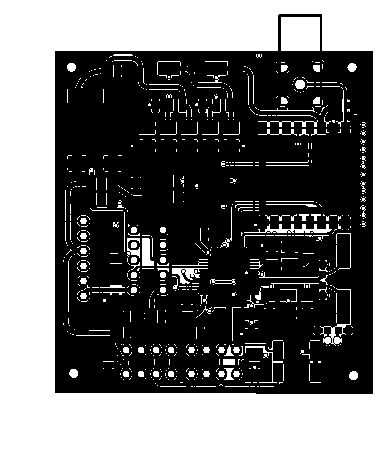
\includegraphics[width=0.7\linewidth]{Assets/PCB_Transmiter.pdf}
	\caption{تصویر برد مدار جاپی طراحی شده برای بخش سنسور.}
	\label{fig:PCBTransmiter}
\end{figure}

\begin{figure}[H]
	\begin{subfigure}[b]{0.5\textwidth}
		\includegraphics[width=\linewidth]{Assets/transmitterBack.png}
		\caption{پشت برد بخش سنسور}
		\label{fig:transmitterBack}
	\end{subfigure}
	\begin{subfigure}[b]{0.5\textwidth}
		\includegraphics[width=\linewidth]{Assets/transmitterFront.png}
		\caption{روی برد بخش سنسور}
		\label{fig:transmitterFront}
	\end{subfigure}
	\caption{تصاویر بردمدارچاپی طراحی‌شده برای بخش سنسور.}
	\label{fig:PCB3dviewtransmitte}
\end{figure}


\قسمت{نحوه ی طراحی بخش ایستگاه}
به طور کلی هدف از طراحی بخش ایستگاه، دریافت داده‌های ارسالی از ماژول لورا و مانیتور کردن آنها در PC می‌باشد. بلوک دیاگرام کلی بخش ایستگاه در شکل \رجوع{fig:Diagram2} نمایش داده شده است.

\begin{figure}[!h]
	\centering
	\includegraphics[width=0.7\linewidth]{Assets/diagram2.pdf}
	\caption{بلوک دیاگرام بخش ایستگاه.}
	\label{fig:Diagram2}
\end{figure}

\noindent
با توجه به بلوک دیاگرام شکل \رجوع{fig:Diagram2} داده‌‌های دریافتی از ماژول لورا توسط میکروکنترلر دریافت شده و توسط پروتکل \متن‌لاتین{USB} به رایانه فرستاده می‌شود و رایانه نیز توسط اپ طراحی شده دیتاهای دریافت شده را دریافت و مانتیور می‌‌کند.


\زیرقسمت{نقشه ی شماتیک بخش ایستگاه}

1- در این بخش که اصلی ترین قسمت مدار می‌باشد از خازن‌های 100 نانوفاراد و 1 میکروفاراد به منظور کاهش نویزهای فرکانس بالا و پایین استفاده شده است. همچنین در تغذیه ی ورودی میکروکنترلر علاوه بر این خازن‌ها از سلف به منظور کاهش ریپل جریان ورودی استفاده شده است. در این بخش از دو عدد کیرستال که یکی برای مدار اصلی و یکی برای قسمت \متن‌لاتین{RTC} استفاده شده است که خازن‌های آن مطابق با دیتاشیت میکروکنترلر انتخاب شده است. همانطور که در شکل مشاهده می‌شود قسمت دیتا و کلاک واحد \متن‌لاتین{I2C} با مقاومت‌های 4٫7 کیلو پول-آپ شده است.

\noindent
2-  این بخش مربوط به ماژول لورا می‌باشد. در این قسمت خازن برای کاهش نویز ورودی به ماژول استفاده شده است و همچنین یک کانکتور برای اتصال آنتن به ماژول قرار داده شده است. 

\noindent
3- در این بخش از یک رگولاتور ‌3٫3 ولت برای تغذیه‌ی ماژول آلتراسونیک استفاده شده است. ورودی رگولاتور،  تغذیه‌ای است که از بیرون به مدار اعمال می‌شود که حداقل می‌بایست 4٫3 ولت باشد و خروجی آن ولتاژ رگوله شده‌ی ‌3٫3 ولت می‌باشد. خازن‌های قرار داده شده در ورودی و خروجی رگولاتور به منظور کاهش ریپل ولتاژ ورودی به رگولاتور و کم کردن نویز خروجی رگولاتور استفاده شده است. همچنین در خروجی این رگولاتور یک دیود نورانی قرار داده شده است که با متصل کردن تغذیه‌ی ورودی روش می‌شود.

\noindent
4- در این بخش از یک کانکتور \متن‌لاتین{MICRO USB} برای برقراری ارتباط بین میکروکنترلر و رایانه استفاده شده است.

\noindent
5- این بخش که یک هدر 1x6 می‌باشد برای پروگرم و دیباگ کردن میکروکنترلر قرار داده شده است.

تصویر بردمدارچاپی طراحی‌شده برای سمت ایستگاه این پروژه در شکل \رجوع{fig:PCB3dviewreceiver} آمده است. همچنین تصاویر شماتیک آن در شکل \رجوع{fig:SchematicReciver} آمده است.
\begin{figure}[H]
	\includegraphics[width=\linewidth]{Assets/Schematic_Reciver.png}
	\caption{تصویر شماتیک برد مدارچاپی سمت ایستگاه.}
	\label{fig:SchematicReciver}
\end{figure}

\begin{figure}[H]
	\centering
	\includegraphics[width=0.7\linewidth]{Assets/PCB_Reciver.pdf}
	\caption{تصویر برد مدار چاپی طراحی شده برای بخش ایستگاه.}
	\label{fig:PCBReciver}
\end{figure}



\begin{figure}[H]
	\begin{subfigure}[b]{0.5\textwidth}
		\includegraphics[width=\linewidth]{Assets/receiverBack.png}
		\caption{پشت برد بخش ایستگاه}
		\label{fig:receiverBack}
	\end{subfigure}
	\begin{subfigure}[b]{0.5\textwidth}
		\includegraphics[width=\linewidth]{Assets/receiverFront.png}
		\caption{روی برد بخش ایستگاه}
		\label{fig:receiverFront}
	\end{subfigure}
	\caption{تصاویر بردمدارچاپی طراحی‌شده برای بخش ایستگاه.}
	\label{fig:PCB3dviewreceiver}
\end{figure}